%-------------------------------------------------------------------------------
%                            BAB II
%               TINJAUAN PUSTAKA DAN DASAR TEORI
%-------------------------------------------------------------------------------
% \fancyhf{} 
% \fancyfoot[R]{\thepage}
\chapter{TINJAUAN PUSTAKA}
%\thispagestyle{plain} % Halaman pertama bab menggunakan gaya plain
\par Untuk memberikan dukungan terhadap penelitian ini, pada bagian ini akan diuraikan beberapa ringkasan teori pendukung yang diambil dari berbagai sumber referensi, seperti buku, artikel, dan karya ilmiah lainnya, termasuk temuan penelitian sebelumnya yang relevan dengan fokus penelitian ini.

\section{Akuisisi Data}

Di dalam dunia industri maupun riset, sistem akuisisi data merupakan ujung terdepan dari proses
pengumpulan data secara mentah langsung dari sumbernya dimana sistem ini mengkonversi data
fisik menjadi data elektronik, akuisisi data merupakan proses awal dalam pengelolaan data, yang melibatkan pengumpulan dan pengambilan data dari berbagai sumber. Proses ini dimulai dengan mengumpulkan data mentah, sepert teks, gambar, dan suara. Data mentah yang dikumpulkan kemudian dikonversi ke dalam format yang dapat diproses oleh sistem komputer atau perangkat lunak yang akan digunakan untuk analisis data. Pada tahap ini, data juga dapat disaring untuk menghilangkan data yang tidak relevan atau tidak valid \citep{pratama2012akuisisi}. 

Data yang telah dikonversi dan disaring ditransmisikan ke sistem/database untuk penyimpanan dan pemrosesan lanjut melalui jaringan atau media penyimpanan fisik. Data tersimpan kemudian diolah dan dianalisis menggunakan berbagai teknik seperti statistik, machine learning, dll. Akuisisi data yang baik menghasilkan data berkualitas tinggi untuk mendukung kesimpulan/tindakan. Dalam penelitian ini, akuisisi dilakukan pada data spasial. Akuisisi data spasial merupakan proses pengambilan data terkait lokasi dan posisi di permukaan bumi. Data spasial terdiri dari data vektor (titik, garis, poligon) dan data raster (\textit{pixel} dari foto udara, pemetaan, citra satelit). Metode akuisisi data spasial antara lain penginderaan jauh, \textit{digital aerial photographs}, \textit{Global Positioning System} (GPS), dan survei pengukuran. Dalam penelitian ini, data raster diambil menggunakan \textit{digital aerial photographs} dari drone, sedangkan data vektor diambil menggunakan GPS. Perbedaan data raster dan data vektor dapat dilihat pada Gambar \ref{vektorkon}.

\begin{figure}[H]
\centering
\frame{\includegraphics [height= 5cm]{image/data vektor titik}}
\caption{Perbedaan data raster dan data vektor
\citep{seputargeografi}}
\label{vektorkon}
\end{figure}

\section{pengindraan Jauh}

\textit{Remote sensing} adalah teknologi yang digunakan untuk mendapatkan informasi mengenai objek atau fenomena di permukaan bumi dari jarak jauh, tanpa perlu melakukan kontak langsung dengan objek tersebut \citep{putri2018analisis}. Teknologi ini dapat dimanfaatkan untuk berbagai keperluan, seperti pemetaan regional, pemantauan lingkungan, dan penelitian ilmiah. Data \textit{remote sensing} dapat dianggap sebagai sumber data yang sangat vital bagi Sistem Informasi Geografis (SIG) karena ketersediaannya secara teratur \citep{ghozali2016pemanfaatan}. Dengan beragam data \textit{remote sensing}, SIG memiliki kemampuan untuk menyediakan informasi yang akurat dan terkini mengenai kondisi permukaan Bumi. Teknologi pengindraan jauh berbasis satelit lebih sering digunakan untuk mengidentifikasi 
sesuatu. Kelebihan dari pengindraan jauh yaitu harganya bisa relatif lebih murah dan 
mudah didapatkan, adanya resolusi temporal (perulangan) hingga bisa digunakan 
untuk pemonitoran, dengan skala yang luas dan bisa menjangkau daerah yang kecil 
atau terpencil, bentuk datanya berupa digital hingga dapat digunakan untuk segala 
keperluan dan akan ditampilkan seperti yang diinginkan \citep{suwargana2010analisis}.

Dengan kemudahan yang ditawarkan oleh teknologi penginderaan jauh dan kehadiran \textit{drone}, proses memperoleh data spasial menjadi semakin mudah. Dalam penelitian ini, data citra udara yang diharapkan memiliki resolusi spasial yang tinggi sehingga dapat memperlihatkan detail objek dengan lebih rinci. Selain itu, diharapkan terdapat \textit{overlap} yang besar antara pasangan foto udara dan akurasi geometrik yang akurat. Citra udara dengan resolusi spasial tinggi dan overlap yang besar memungkinkan rekonstruksi model 3D permukaan bumi dengan ketelitian yang lebih baik. Akurasi geometrik yang akurat juga diperlukan untuk memastikan posisi objek di permukaan bumi dapat ditentukan dengan tepat dalam pengolahan data spasial selanjutnya.



\section{UAV (\textit{Unmanned Aerial Vehicle})}

\par \textit{Unmanned Aerial Vehicles} (UAV), yang lebih umum dikenal sebagai "\textit{Drone}", 
juga disebut sebagai robot terbang yang melibatkan pesawat udara tanpa awak (UAV) 
yang dapat terbang dalam jarak ribuan kilometer maupun \textit{drone} kecil yang terbang di
area terbatas. \textit{Drone} merupakan platform pemantauan jarak jauh yang baru, ekonomis, 
dan mudah digunakan, memberikan pengguna berbagai opsi terkait lokasi, waktu, dan 
metode pengumpulan citra serta data geospasial. pada penelitian ini drone yang digunakan adalah DJI Phantom 4 Pro yang dapat dilihat pada Gambar \ref{gambardrone}

% Menambahkan gambar 
\begin{figure}[H]
\centering
\frame{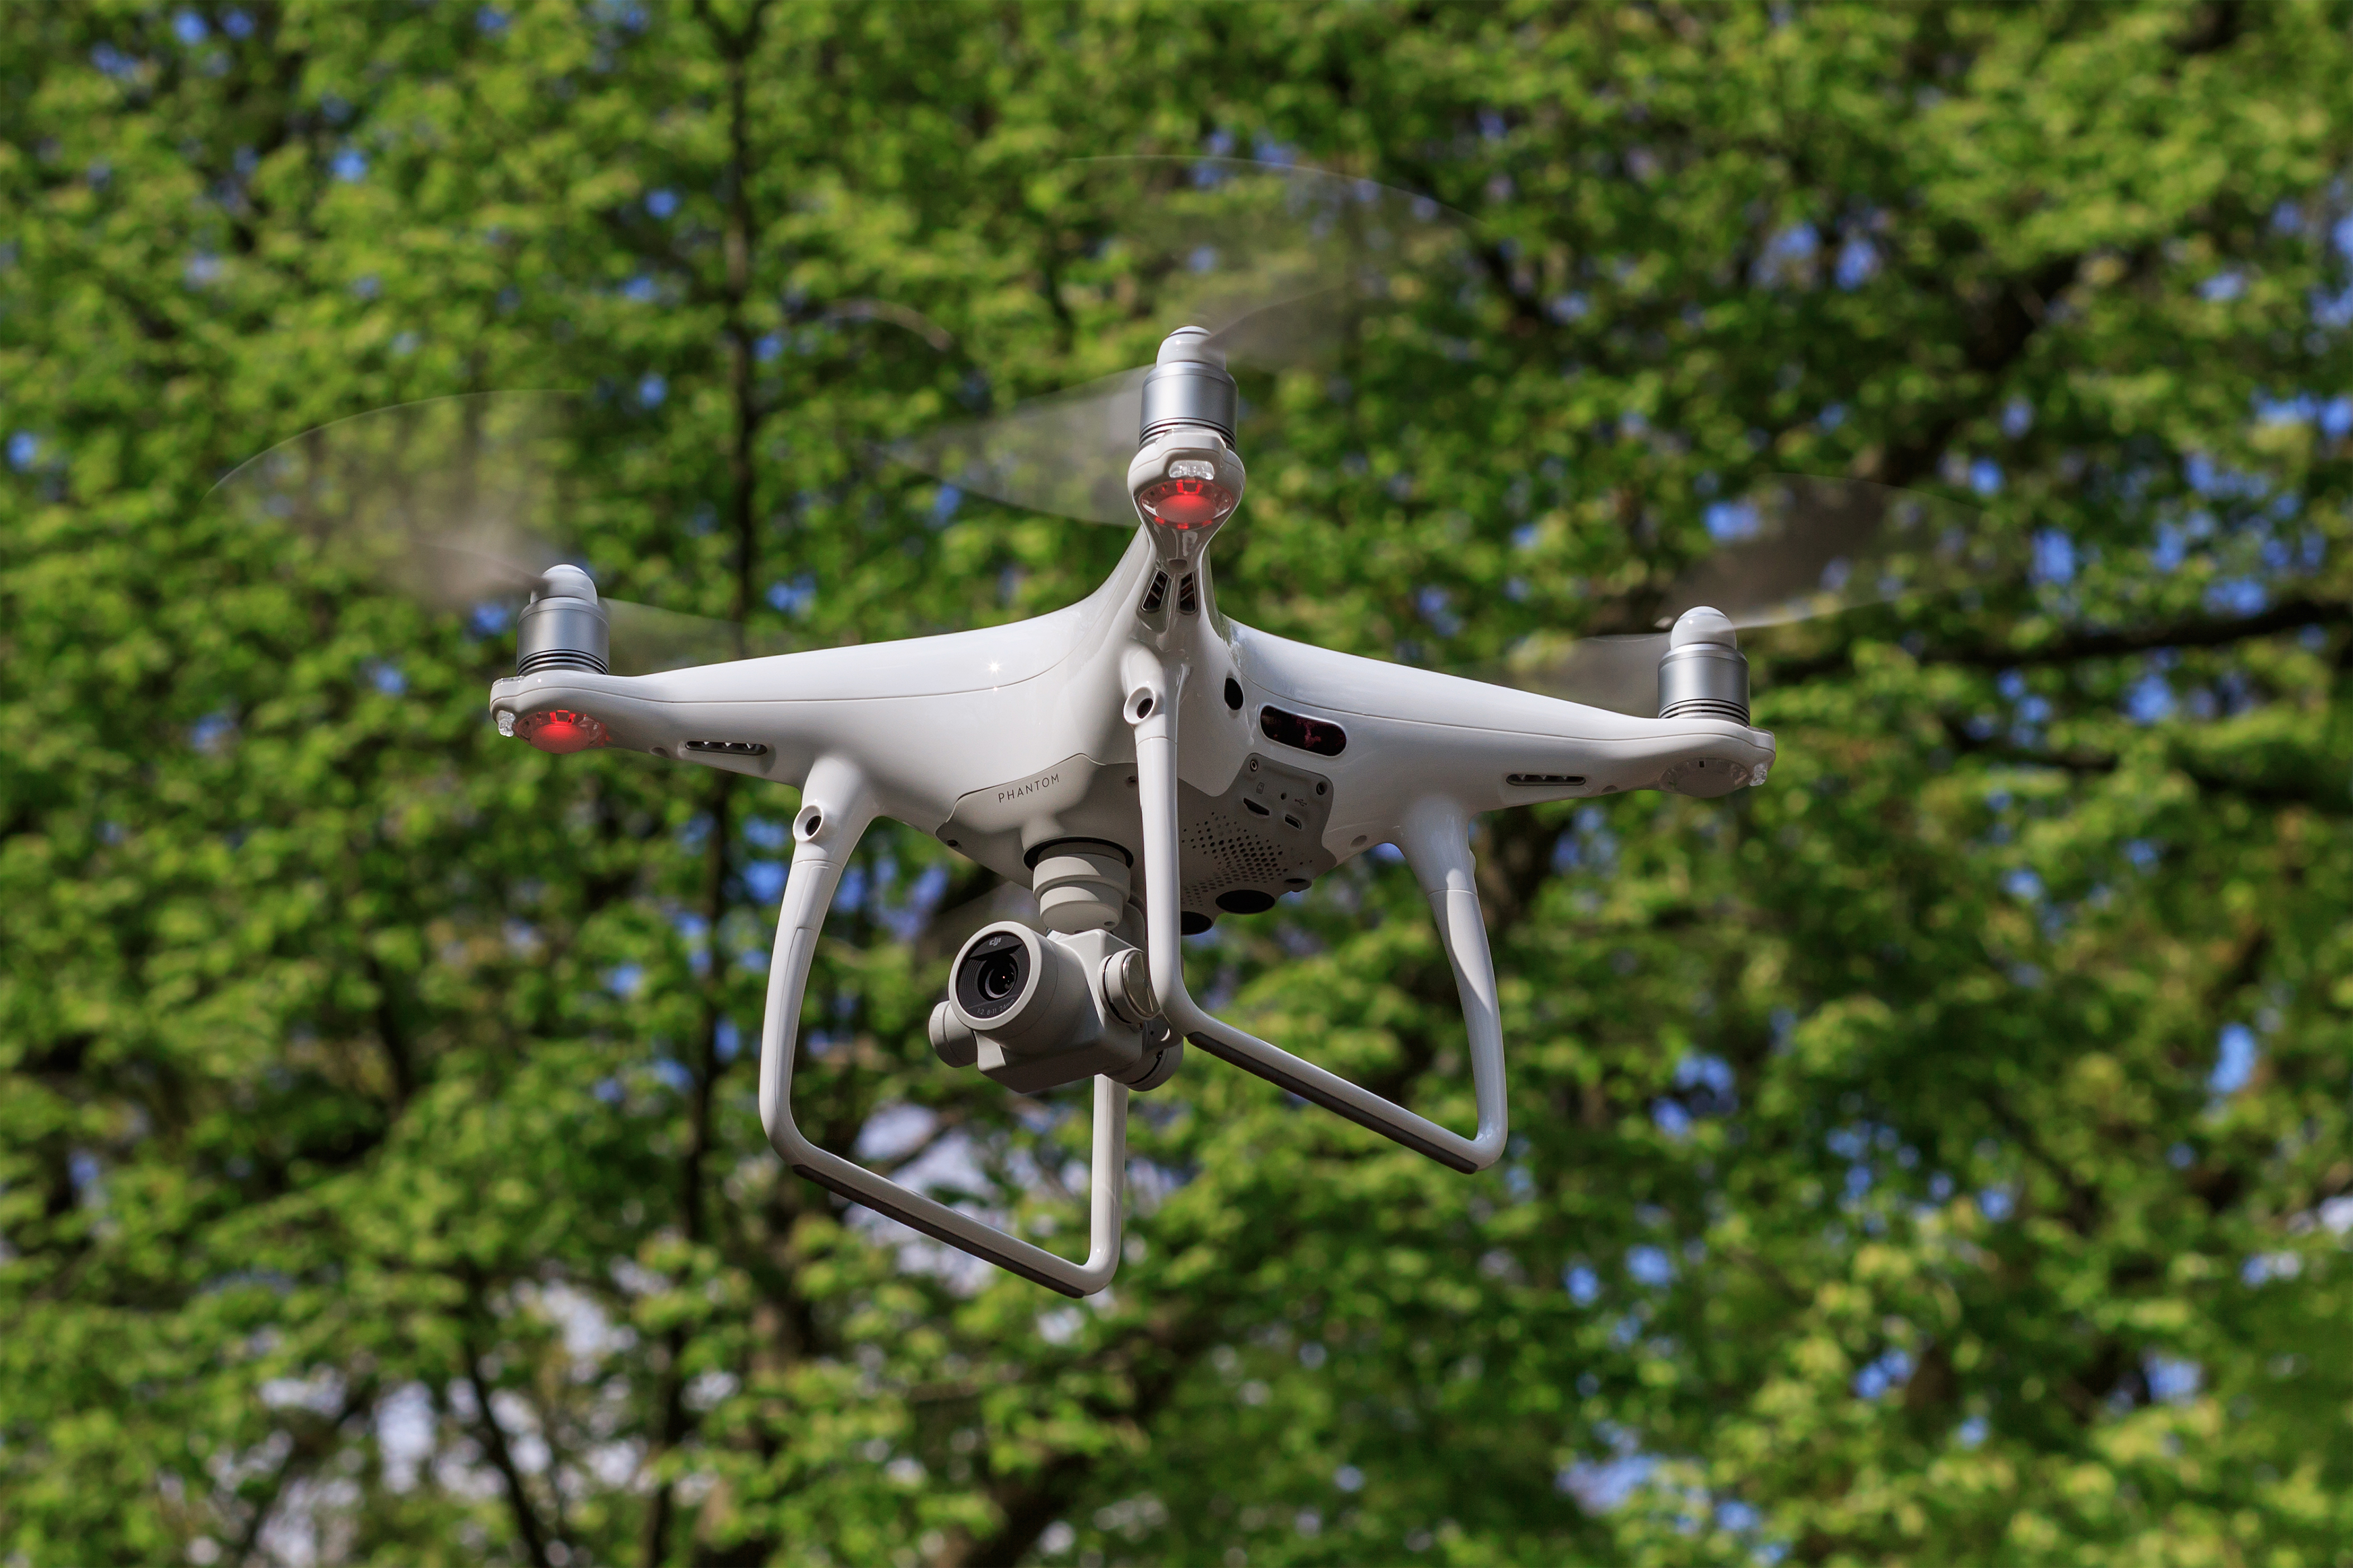
\includegraphics [height= 5cm]{image/DJI}}
\caption{\textit{Drone} DJI Phantom 4 Pro}
\label{gambardrone}
\end{figure}

\par \textit{Drone} telah menjadi alat yang sangat berharga dalam pemantauan jarak jauh dan pemetaan, menawarkan karakteristik unik dalam hal spasial, temporal, dan spektral. Salah satu keunggulan utama dalam hal spasial \textit{drone} adalah kemampuannya menghasilkan data dengan resolusi spasial yang sangat tinggi, memungkinkan pengumpulan informasi dengan tingkat detail yang luar biasa. Sebagai contoh, drone seperti DJI Phantom 4 Pro mampu mencapai resolusi spasial hingga 2,40 cm/pixel pada ketinggian terbang 90 meter \citep{hernina2019analisis}, suatu kemampuan yang sangat bermanfaat dalam pemetaan bidang tanah dan survei lapangan. Resolusi spasial yang optimal ini menjadikan \textit{drone} sebagai pelengkap ideal untuk metode survei konvensional, memungkinkan pembuatan peta lahan yang sangat akurat dan terperinci. Hubungan antara ketinggian terbang dan resolusi spasial yang dihasilkan dapat dilihat melalui tabel \ref{resolusispasial} yang menunjukkan resolusi spasial pada berbagai ketinggian menggunakan DJI Phantom 4 Pro, memberikan panduan berharga bagi para praktisi dalam merencanakan pemetaan mereka.

\begin{table}[H]
\centering
\caption{Resolusi spasial berdasarkan ketinggian terbang yang dapat dihasilkan pada Drone DJI Phantom 4 Pro \citep{hernina2019analisis}}
\label{resolusispasial}
\begin{tabular}{|l|l|l|}
\hline
\textbf{No.} & \textbf{Tinggi Terbang} & \textbf{Resolusi Spasial (cm/pixel)} \\ \hline
1.           & 90                      & 2,40                                 \\ \hline
2.           & 110                     & 2,97                                 \\ \hline
3.           & 130                     & 3,52                                 \\ \hline
4.           & 150                     & 4,09                                 \\ \hline
\end{tabular}
\end{table}

\par Drone tidak hanya unggul dalam aspek spasial, tetapi juga menawarkan keunggulan dalam karakteristik temporal dan spektral. Dari segi temporal, \textit{drone} memiliki kemampuan luar biasa dalam pengumpulan data secara \textit{real-time} dan efisien. Dengan kemampuan terbang dan mengakuisisi data dalam waktu yang relatif singkat, \textit{drone} menjadi solusi ideal untuk aplikasi survei lapangan yang membutuhkan data cepat dan akurat. Sementara itu, karakteristik spektral \textit{drone} memungkinkan pengumpulan data dalam berbagai spektrum elektromagnetik. Sebagai contoh, \textit{drone} seperti DJI Phantom 4 Pro dilengkapi dengan sensor kamera digital beresolusi tinggi 12 Megapixel, yang mampu menghasilkan data dengan tingkat detail yang mengesankan. Keunggulan ini terbukti dalam aplikasi pemetaan bidang tanah, di mana \textit{drone} menghasilkan orthofoto dengan ketelitian geometri yang sangat tinggi, menunjukkan perbedaan yang tidak signifikan dibandingkan dengan metode konvensional. Kombinasi karakteristik temporal dan spektral ini menjadikan \textit{drone} sebagai alat yang sangat efektif dan efisien dalam berbagai aplikasi pemetaan dan survei modern.

\textit{Drone} profesional untuk pemetaan juga dilengkapi dengan beragam jenis kamera canggih yang dirancang khusus untuk menghasilkan data berkualitas tinggi dan presisi. Kamera RGB standar dengan resolusi tinggi, biasanya mulai dari 12MP hingga 100MP atau lebih, merupakan pilihan umum untuk menghasilkan gambar berwarna natural dengan detail yang tajam. Untuk aplikasi yang lebih spesifik, kamera multispektral dan hiperspektral menjadi pilihan utama. Kamera multispektral, yang menangkap data dalam beberapa band spektral termasuk inframerah dekat (NIR), sangat bermanfaat untuk analisis vegetasi dan pertanian presisi. Sementara itu, kamera hiperspektral, dengan kemampuannya mengumpulkan data dalam ratusan band spektral yang sangat sempit, ideal untuk analisis mineral dan aplikasi lingkungan yang kompleks.

Selain itu, \textit{drone} profesional juga sering dilengkapi dengan kamera termal untuk menangkap data suhu permukaan, yang berguna dalam inspeksi bangunan dan pemantauan kebakaran hutan. Teknologi LiDAR (\textit{Light Detection and Ranging}) juga semakin populer dalam pemetaan \textit{drone}, menggunakan laser untuk menghasilkan model elevasi digital yang sangat akurat, ideal untuk pemetaan topografi dan pemodelan 3D perkotaan. Untuk aplikasi khusus seperti pemodelan 3D perkotaan dan inspeksi infrastruktur, kamera oblique yang dapat mengambil gambar dari berbagai sudut menjadi pilihan yang tepat. Terakhir, kamera 360° juga mulai digunakan dalam \textit{drone} pemetaan untuk menghasilkan gambar panorama yang berguna dalam pembuatan virtual tour dan dokumentasi lokasi secara komprehensif. Pemilihan jenis kamera pada \textit{drone} profesional untuk pemetaan sangat bergantung pada tujuan spesifik proyek, kondisi lingkungan, dan kebutuhan data yang ingin diperoleh, dengan banyak platform \textit{drone} modern memungkinkan penggantian payload untuk fleksibilitas maksimal.


\section{Perencanaan jalur terbang \textit{Drone}}

Perencanaan jalur terbang \textit{drone} merupakan aspek krusial dalam pemetaan fotogrametri. Perencanaan yang tepat sangat penting untuk menghasilkan data pemetaan yang akurat dan efisien, dengan mempertimbangkan faktor-faktor seperti luas area, resolusi yang diinginkan, dan prosedur yang ditentukan, karena jika ada salah satu tahap pembuatan jalur terbang yang terlewat maka akan mempengaruhi hasil akhir \citep{guntara2015perencanaan}. Salah satu metode yang digunakan dalam perancangan jalur terbang adalah metode waypoint. Metode ini melibatkan penentuan titik-titik koordinat yang akan dilalui oleh \textit{drone} selama penerbangan, memungkinkan kontrol yang lebih presisi atas rute penerbangan dan area cakupan. Dalam berbagai aplikasi, pemanfaatan data \textit{drone} telah dikaji untuk berbagai bidang. Desain jalur terbang yang tepat sangat penting untuk menghasilkan data yang akurat dalam pemetaan area, inventarisasi objek, dan pemantauan kondisi lingkungan. Untuk berbagai jenis wilayah, optimalisasi perencanaan jalur terbang UAV perlu mempertimbangkan kondisi topografi, batasan regulasi, dan faktor lingkungan seperti angin. Untuk area dengan topografi yang bervariasi, penggunaan mode penerbangan \textit{terrain following} disarankan, di mana \textit{drone} menjaga ketinggian relatif yang konstan terhadap permukaan tanah. Pendekatan ini memungkinkan adaptasi terhadap berbagai kondisi lapangan dan memastikan kualitas data yang konsisten.

Faktor-faktor yang mempengaruhi kualitas hasil pemetaan juga perlu diperhatikan dalam desain jalur terbang. Analisis menunjukkan beberapa temuan penting. Pertama, ketinggian terbang berbanding terbalik dengan ketelitian peta, di mana semakin rendah ketinggian terbang, semakin tinggi ketelitian yang dihasilkan. Kedua, kecepatan \textit{Drone} yang lebih rendah cenderung menghasilkan peta yang lebih teliti, meskipun hal ini perlu diimbangi dengan pertimbangan efisiensi waktu penerbangan. Terakhir, \textit{overlap} foto memiliki pengaruh signifikan, dengan \textit{overlap} yang lebih besar (80\% frontal \textit{overlap} dan 60\% - 70\% \textit{side overlap}) menghasilkan ketelitian yang lebih baik dibandingkan dengan overlap yang lebih kecil dan lebih membantu dalam proses stitching foto dan meningkatkan akurasi rekonstruksi 3D \citep{torres2018assessing}. Dalam aspek regulasi, penting untuk memperhatikan peraturan penerbangan drone yang berlaku di Indonesia, termasuk batas ketinggian maksimum dan area terbang yang diizinkan, Dengan mempertimbangkan semua faktor ini, desain jalur terbang yang optimal dapat menghasilkan data pemetaan yang akurat dan efisien, sesuai dengan kebutuhan spesifik proyek dan kondisi lapangan di Indonesia.

\section{Mosaik}

\par Mosaik citra spasial yang diambil menggunakan \textit{drone} melibatkan serangkaian proses kompleks yang terjadi di latar belakang aplikasi. Proses ini dimulai dengan akuisisi citra, di mana drone mengambil serangkaian foto yang tumpang tindih, biasanya dengan overlap 60-80\% untuk memastikan area yang cukup untuk pencocokan fitur. Setelah citra diperoleh, langkah berikutnya adalah ekstraksi dan pencocokan fitur. Dalam tahap ini, algoritma \textit{computer vision} seperti SIFT atau SURF digunakan untuk mengidentifikasi dan mencocokkan fitur-fitur unik antar citra yang tumpang tindih seperti yang terlihat pada Gambar \ref{mosaik}, memungkinkan aplikasi untuk menentukan hubungan spasial antar citra \citep{ghosh2016survey}.

\begin{figure}[H]
\centering
\frame{\includegraphics [height= 5cm]{image/mosaik}}
\caption{Ilustrasi proses mosaik pada citra udara}
\label{mosaik}
\end{figure}

Dalam proses ekstraksi dan pencocokan fitur, dua algoritma \textit{computer vision} yang sering digunakan adalah SIFT (\textit{Scale-Invariant Feature Transform}) dan SURF (\textit{Speeded Up Robust Features}). SIFT yang diperkenalkan oleh Lowe pada tahun 1999, adalah algoritma yang mampu mendeteksi dan mendeskripsikan fitur lokal dalam gambar. Keunggulan utama SIFT terletak pada kemampuannya untuk mengenali fitur yang \textit{invariant} terhadap skala, rotasi, dan sebagian besar terhadap perubahan pencahayaan dan sudut pandang 3D. Ini membuat SIFT sangat cocok untuk pencocokan fitur dalam citra drone yang diambil dari berbagai sudut dan ketinggian \citep{lowe2004distinctive}. Di sisi lain, SURF, yang dikembangkan oleh Bay et al. pada tahun 2006, dirancang sebagai versi yang lebih cepat dan lebih efisien dari SIFT. Meskipun sedikit kurang akurat dibandingkan SIFT dalam beberapa kasus, SURF umumnya lebih cepat dan masih cukup tangguh untuk banyak aplikasi pembuatan mosaik citra drone \citep{bay2006surf}.

Meskipun proses ini umumnya otomatis, tantangan seperti variasi pencahayaan, pergerakan objek, dan kompleksitas \textit{terrain} dapat mempengaruhi kualitas hasil akhir. Namun, pengembangan terbaru dalam \textit{machine learning} dan \textit{computer vision} terus meningkatkan akurasi dan efisiensi proses mosaik, menjanjikan hasil yang lebih baik di masa depan.


\section{\textit{Ground Control Point} (GCP)}

 GCP (\textit{Ground Control Point}) atau titik kontrol tanah adalah penandaan tempat yang terkoordinasi dalam bentuk beberapa titik yang diperlukan untuk mengoreksi data dan meningkatkan citra umum, yang disebut proses koreksi GCP, terdiri dari sepasang X dan koordinat Y yang terdiri dari koordinat asal dan referensi koordinat. Keakuratan GCP sangat bergantung pada jenis GPS yang digunakan dan jumlah sampel GCP di lokasi dan waktu pengambilan \citep{widodo2023pemanfaatan}. Dalam pemetaan menggunakan \textit{drone}, \textit{Ground Control Points} (GCP) menjadi elemen kunci untuk memastikan akurasi dan konsistensi hasil. Meskipun \textit{drone} dilengkapi dengan sensor GPS, seringkali tidak dapat memberikan akurasi yang memadai untuk aplikasi pemetaan yang presisi. Melalui pemasangan GCP di area yang akan dipetakan, kita dapat memperbaiki distorsi geometrik pada citra \textit{drone} dan menjamin bahwa citra tersebut terdaftar dengan benar ke koordinat geografis yang tepat. Hal ini tidak hanya meningkatkan akurasi pemetaan secara keseluruhan, tetapi juga memungkinkan perbandingan dan analisis yang konsisten antara citra dari berbagai penerbangan atau sumber data. Dengan demikian, penggunaan GCP menjadi suatu keharusan dalam pemetaan menggunakan \textit{drone} untuk aplikasi yang memerlukan presisi dan konsistensi spasial yang tinggi. berikut contoh \textit{Ground Control Point} (GCP) yang digunakan dalam proses pemetaan yang ditampilkan pada Gambar 2.3.

 \begin{figure}[H]
\centering
\frame{\includegraphics [height= 5cm]{image/x-gcp-contour-lines}}
\caption{\textit{Ground Control Point} di lapangan survei}
\label{dig_facenet}
\end{figure}

\section{Matriks Evaluasi}

\par Matriks evaluasi pada mosaik citra memberikan informasi kuantitatif tentang akurasi geometrik. Kombinasi beberapa matriks evaluasi ini memungkinkan perbandingan yang komprehensif antara hasil mosaik dari berbagai perangkat lunak atau metode pemrosesan yang berbeda.

\subsection{\textit{Root Mean Square Error} (RMSE)}
    \textit{Root Mean Square Error} (RMSE) merupakan metrik evaluasi yang umum digunakan untuk mengukur akurasi hasil mosaik citra spasial, terutama yang diperoleh dari pencitraan drone. Dalam konteks pemetaan drone, kita sering menggunakan dua jenis RMSE, yaitu RMSEr untuk akurasi horizontal dan RMSEz untuk akurasi vertikal. RMSEr (\textit{Root Mean Square Error radial}) mengukur akurasi posisional horizontal dengan menggabungkan error dalam arah x (longitude) dan y (latitude), sedangkan RMSEz (\textit{Root Mean Square Error in} z) mengukur akurasi vertikal atau elevasi. RMSE menghitung rata-rata perbedaan kuadrat antara nilai yang diprediksi (dalam hal ini, koordinat piksel pada citra mosaik) dan nilai yang sebenarnya (koordinat referensi di lapangan), kemudian mengambil akar kuadratnya. Dalam konteks mosaik citra \textit{drone}, RMSE digunakan untuk menilai sejauh mana citra hasil mosaik menyimpang dari posisi sebenarnya di permukaan bumi. Semakin rendah nilai RMSE, semakin tinggi akurasi geometris dari mosaik yang dihasilkan. RMSE dan RMSEr dihitung dengan rumus seperti pada Gambar \ref{rumus_rmse}, \ref{rumus_rmser} berikut:

    \begin{figure}[H]
    \centering
    \frame{\includegraphics [height= 2cm]{image/RMSE1.jpg}}
    \caption{Rumus Root Mean Square Error \citep{geeksforgeeksRMSE}}
    \label{rumus_rmse}
    \end{figure}

    \begin{figure}[H]
    \centering
    \frame{\includegraphics [height= 2cm]{rumusrmser.png}}
    \caption{Rumus Root Mean Square Error Radial (RMSEr)}
    \label{rumus_rmser}
    \end{figure}
    
    Seperti yang terlihat pada Gambar \ref{rumus_rmse} yang mana '\textit{predicted}' adalah koordinat pada citra mosaik, '\textit{actual}' adalah koordinat referensi di lapangan, dan 'n' adalah jumlah titik sampel \citep{jaud2016assessing}. Penggunaan RMSE dalam evaluasi mosaik citra drone telah banyak diterapkan dalam berbagai studi. Misalnya, dalam pemetaan topografi menggunakan citra drone, RMSE horizontal berkisar antara 5,5 cm hingga 6,9 cm, tergantung pada ketinggian terbang drone \citep{aguera2017assessment}. RMSE juga digunakan untuk membandingkan akurasi mosaik citra yang dihasilkan dari berbagai perangkat lunak fotogrametri. Penelitian menunjukkan bahwa pemilihan perangkat lunak dan metode pengolahan dapat mempengaruhi nilai RMSE akhir dari mosaik yang dihasilkan \citep{padro2019comparison}. 
    

%     \begin{table}[h]
% \centering
% \caption{Skala Peta Dasar dan Nilai GSD}
% \begin{tabular}{|c|c|}
% \hline
% Skala Peta Dasar & Nilai GSD (cm) \\
% \hline
% 1:10.000 & $\leq$ 30 \\
% \hline
% 1:5.000 & $\leq$ 15 \\
% \hline
% 1:2.500 & $\leq$ 10 \\
% \hline
% 1:1.000 & $\leq$ 8 \\
% \hline
% \end{tabular}
% \label{tab:skala-gsd}
% \end{table}

\subsection{\textit{Circular Error} 90\% (CE90) dan \textit{Linear Error} 90\% (LE90)}

    \textit{Circular Error} (CE90) dan \textit{Linear Error} (LE90) merupakan parameter penting dalam mengevaluasi akurasi geometrik dari citra hasil pemetaan udara, termasuk mosaik citra yang dihasilkan dari pengambilan gambar menggunakan \textit{drone}. Kedua parameter ini sering digunakan untuk mengukur tingkat presisi posisional dari data geospasial. \textit{Circular Error} 90 (CE90) didefinisikan sebagai radius lingkaran yang mencakup 90\% dari titik-titik data yang diukur relatif terhadap posisi sebenarnya. Dalam konteks mosaik citra drone, CE90 menggambarkan akurasi horizontal dari citra yang dihasilkan. Semakin kecil nilai CE90, semakin tinggi akurasi posisional horizontal citra tersebut \citep{peppa2019photogrammetric}. \textit{Linear Error} 90 (LE90), di sisi lain, mengukur akurasi vertikal. LE90 didefinisikan sebagai interval vertikal yang mencakup 90\% dari perbedaan elevasi antara titik-titik yang diukur dengan nilai elevasi sebenarnya. Dalam konteks mosaik citra drone, LE90 sangat penting untuk menilai akurasi model elevasi digital yang dihasilkan dari data penginderaan jauh \citep{wolf2002elementary}. CE90 dan LE90 dihitung menggunakan rumus seperti pada Gambar \ref{rumus_ce}.

    \begin{figure}[H]
    \centering
    \frame{\includegraphics [height= 2cm]{rumus cele.png}}
    \caption{Rumus CE90 dan LE90 \citep{BIG2014}}
    \label{rumus_ce}
    \end{figure}

    Penggunaan CE90 dan LE90 dalam evaluasi mosaik citra drone memungkinkan penilaian yang lebih komprehensif terhadap kualitas geometrik hasil pemetaan. Studi menunjukkan bahwa penggunaan \textit{drone} dengan sensor kamera beresolusi tinggi dapat menghasilkan mosaik ortofoto dengan CE90 kurang dari 10 cm dan LE90 kurang dari 15 cm, mendemonstrasikan potensi tinggi dari teknologi \textit{drone} untuk pemetaan presisi tinggi \citep{kalantar2017drone}. Namun, perlu dicatat bahwa akurasi yang dicapai dapat bervariasi tergantung pada berbagai faktor seperti kualitas kamera, ketinggian terbang, kondisi cuaca, dan metode pengolahan data. Oleh karena itu, analisis CE90 dan LE90 penting dilakukan dalam setiap proyek pemetaan drone \citep{sanz2018accuracy}. Penting untuk dicatat bahwa interpretasi CE90 dan LE90 harus mempertimbangkan resolusi spasial citra asli dan skala peta yang diinginkan.

    Di Indonesia, standar ketelitian peta diatur oleh Badan Informasi Geospasial (BIG) melalui Peraturan Kepala BIG Nomor 6 Tahun 2018 tentang Pedoman Teknis Ketelitian Peta Dasar seperti pada Tabel \ref{tab:ketelitian-peta-rbi}. Standar ini penting diperhatikan dalam pembuatan mosaik citra dari drone untuk memastikan hasil pemetaan memenuhi kriteria ketelitian nasional.

    \begin{table}[h]
\centering
\caption{Ketelitian Peta RBI}
\label{tab:ketelitian-peta-rbi}
\resizebox{\textwidth}{!}{
\begin{tabular}{|c|c|c|c|c|c|c|c|c|}
\hline
\multirow{3}{*}{No} & \multirow{3}{*}{Skala} & \multirow{3}{*}{\begin{tabular}[c]{@{}c@{}}Interval\\ Kontur\\ (m)\end{tabular}} & \multicolumn{6}{c|}{Ketelitian Peta RBI} \\
\cline{4-9}
 &  &  & \multicolumn{2}{c|}{Kelas 1} & \multicolumn{2}{c|}{Kelas 2} & \multicolumn{2}{c|}{Kelas 3} \\
\cline{4-9}
 &  &  & \begin{tabular}[c]{@{}c@{}}Horisontal\\ (CE90\\ dalam m)\end{tabular} & \begin{tabular}[c]{@{}c@{}}Vertikal\\ (LE90\\ dalam\\ m)\end{tabular} & \begin{tabular}[c]{@{}c@{}}Horisontal\\ (CE90\\ dalam m)\end{tabular} & \begin{tabular}[c]{@{}c@{}}Vertikal\\ (LE90\\ dalam m)\end{tabular} & \begin{tabular}[c]{@{}c@{}}Horisontal\\ (CE90\\ dalam m)\end{tabular} & \begin{tabular}[c]{@{}c@{}}Vertikal\\ (LE90\\ dalam\\ m)\end{tabular} \\
\hline
1 & 1:1.000.000 & 400 & 300 & 200 & 600 & 300 & 900,0 & 400 \\
\hline
2 & 1:500.000 & 200 & 150 & 100 & 300 & 150 & 450,0 & 200 \\
\hline
3 & 1:250.000 & 100 & 75 & 50 & 150 & 75 & 225,0 & 100 \\
\hline
4 & 1:100.000 & 40 & 30 & 20 & 60 & 30 & 90,0 & 40 \\
\hline
5 & 1:50.000 & 20 & 15 & 10 & 30 & 15 & 45,0 & 20 \\
\hline
6 & 1:25.000 & 10 & 7,5 & 5 & 15 & 7,5 & 22,5 & 10 \\
\hline
7 & 1:10.000 & 4 & 3 & 2 & 6 & 3 & 9,0 & 4 \\
\hline
8 & 1:5.000 & 2 & 1,5 & 1 & 3 & 1,5 & 4,5 & 2 \\
\hline
9 & 1:2.500 & 1 & 0,75 & 0,5 & 1,5 & 0,75 & 2,3 & 1 \\
\hline
10 & 1:1.000 & 0,4 & 0,3 & 0,2 & 0,6 & 0,3 & 0,9 & 0,4 \\
\hline
\end{tabular}
}
\end{table}

    






\section{Penelitian Terkait}

\par Penelitian yang dilakukan oleh Petrus Krisologus Hamur dkk.(2019) yang membahas tentang "Kajian pengolahan data foto udara menggunakan perangkat lunak Agisoft Photoscan dan PIX4D Mapper". Dalam penelitian ini, pemrosesan data foto udara dilakukan menggunakan perangkat lunak Agisoft Photoscan dan Pix4D Mapper, melibatkan sebanyak 158 foto dan 8 titik \textit{Ground Control Point} (GCP). Untuk menguji akurasi posisi horizontal dan vertikal, akan diterapkan metode perhitungan yang diacu dari Peraturan Badan Informasi Geospasial (BIG) No. 15 tahun 2014. Sementara itu, uji ketelitian objek pada Orthofoto akan melibatkan interpretasi dan perhitungan dengan menerapkan metode persamaan omisi komisi. Dari hasil penelitian akurasi data \textit{Digital Elevation Model} (DEM) dan Orthofoto, dengan merujuk pada standar yang ditetapkan dalam Peraturan BIG No. 15 tahun 2014, ditemukan bahwa nilai \textit{Linear Error} 90\% (LE90) dari Agisoft Photoscan adalah sekitar 0.279 m, sedangkan Pix4D Mapper mencapai 0.509 m. Demikian pula, nilai \textit{Circular Error} 90\% (CE90) dari Agisoft Photoscan adalah sekitar 0.139 m, sementara Pix4D Mapper sebesar 0.224 m. Lebih lanjut, dalam menguji akurasi objek dari data Orthofoto menggunakan metode omisi komisi, hasil perhitungan menunjukkan bahwa presentase rata-rata akurasi objek dari kedua perangkat lunak, Agisoft Photoscan dan Pix4D Mapper, melebihi 90\%. Keakuratan ini memenuhi standar yang disyaratkan, yaitu lebih dari 85\%. Penelitian ini secara keseluruhan memberikan pemahaman yang mendalam mengenai kemampuan Agisoft Photoscan dan Pix4D Mapper dalam menghasilkan data DEM dan Orthofoto yang memenuhi kriteria akurasi geometri dan objek yang telah ditetapkan \citep{hamur2019kajian}.

Penelitian yang dilakukan oleh Sultan Alifian Hapriansyah dkk. (2021) yang membahas tentang "Analisis perbandingan ketelitian hasil orthomosaic menggunakan perangkat lunak komersial PIX4Dmapper dan open source WebODM" yang menyajikan penelitian dan hasil sebagai berikut. Foto tegak merupakan hasil pengambilan gambar dari pesawat atau UAV yang memiliki sumbu optik kamera yang berorientasi vertikal atau hampir vertikal. Orthomosaic, yang diperoleh dari pengolahan foto udara menggunakan perangkat lunak fotogrametri khusus, menjadi fokus dalam penelitian ini. Penelitian ini menggunakan data foto udara dan GPS wilayah Kebonwaris, Kecamatan Pandaan, Pasuruan - Jawa Timur. WenODM dan versi uji coba Pix4Dmapper digunakan sebagai perangkat lunak pembanding. Proses pengolahan data dimulai dari langkah-langkah impor gambar, impor titik kontrol, pembentukan awan titik, pembentukan mesh, pembentukan model permukaan, hingga pembentukan orthomosaic. Pix4Dmapper memberikan nilai \textit{Root Mean Square Error} (RMSe) horizontal sekitar 0,67361672 dan RMSe vertikal sekitar 0,664288006. Sementara itu, WebODM memberikan nilai ketelitian dengan RMSe horizontal sekitar 1,92810327 dan RMSe vertikal sekitar 1,195321336. Resolusi yang diperoleh dari WebODM adalah sekitar 5,5cm/piksel, sedangkan Pix4Dmapper sekitar 6,4cm/piksel. Dari hasil analisis, dapat disimpulkan bahwa Pix4Dmapper unggul dalam hal ketelitian yang diperoleh, sementara WebODM memiliki keunggulan dalam resolusi \citep{hapriansyah2021analisis}.

Penelitian yang dilakukan oleh Hadiwijaya Lesmana Salim dkk. (2018) yang membahas tentang "Pemetaan dinamika hutan mangrove menggunakan \textit{drone} dan pengindraan jauh di P. Rambut, Kepulauan Seribu" yang menyajikan penelitian dan pengamatan terhadap sebaran dan luas hutan mangrove di Pulau Rambut Pada bulan November 2017 dan Juli 2010. Pengamatan ini melibatkan analisis foto udara dan citra Geo Eye 1. Untuk memvalidasi data lapangan, dilakukan kunjungan lapangan. Metode yang diterapkan dalam penelitian ini adalah segementasi dan klasifikasi terbimbing menggunakan pendekatan analisis berbasis objek (OBIA). Berdasarkan hasil analisis foto udara, data citra, dan validasi lapangan, dapat diestimasi bahwa pada tahun 2010, luas hutan mangrove di Pulau Rambut mencapai 16,73 ha, sementara pada tahun 2017 mencapai 17,48 ha, menunjukkan peningkatan sebesar 0,75 ha. Hutan mangrove di Pulau Rambut terdiri dari 10 jenis, dengan dominasi jenis \textit{Rhizophora mucronata}. Penelitian ini menyimpulkan bahwa analisis berbasis objek terhadap foto udara yang diambil dengan \textit{drone} menghasilkan pemetaan dinamika hutan mangrove yang lebih baik dibandingkan dengan penggunaan citra satelit Geo Eye 1. Akurasi keseluruhan mencapai 77,3\%, dan nilai koefisien kappa sebesar 0,62 \citep{islands2018pemetaan}.
% \fancyhf{} 
% \fancyfoot[R]{\thepage}

\begin{comment}
\bibliography{daftar-pustaka}
\end{comment}
